\section{Rekombination}\label{recombination}

% http://www.geatbx.com/docu/options-03.html
% http://citeseerx.ist.psu.edu/viewdoc/download?doi=10.1.1.61.6575&rep=rep1&type=pdf
% http://chern.ie.nthu.edu.tw/alg2003/chap-8-9.pdf
% http://siebn.de/download/GenetischeAlgorithmen.pdf

\paragraph{Order Crossover (OX)} von L. Davis
Beschreibung

\begin{figure}[h!]
  \centering
  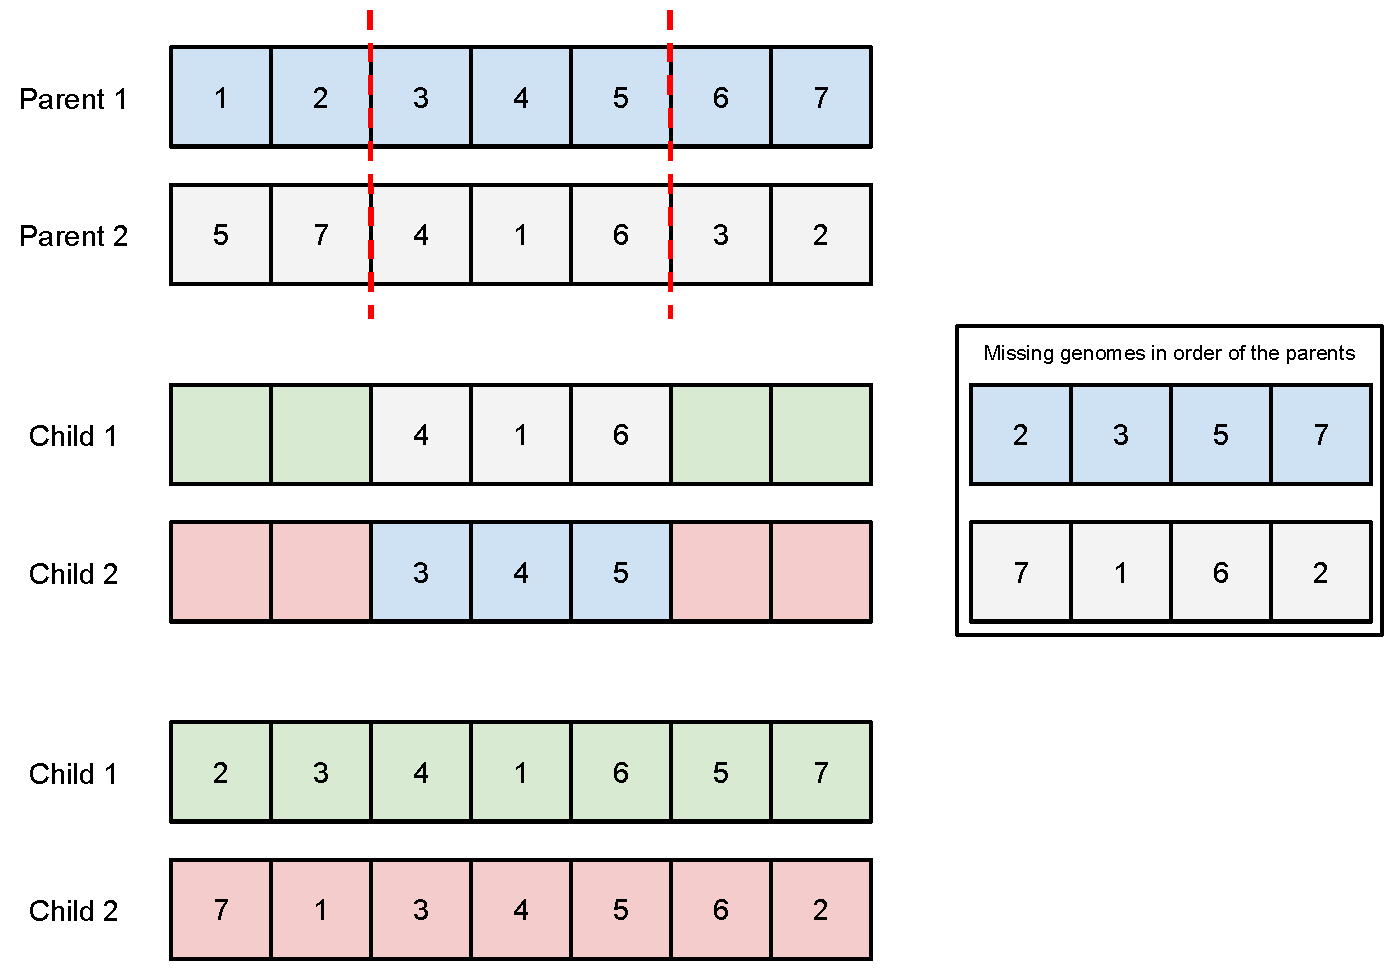
\includegraphics[width=1.0\textwidth]{Figures/recox.pdf}
  \caption{Order Crossover (OX)}\label{fig.recox}
\end{figure}


\paragraph{Partially matched Crossover (recpm)}

\begin{figure}[h!]
  \centering
  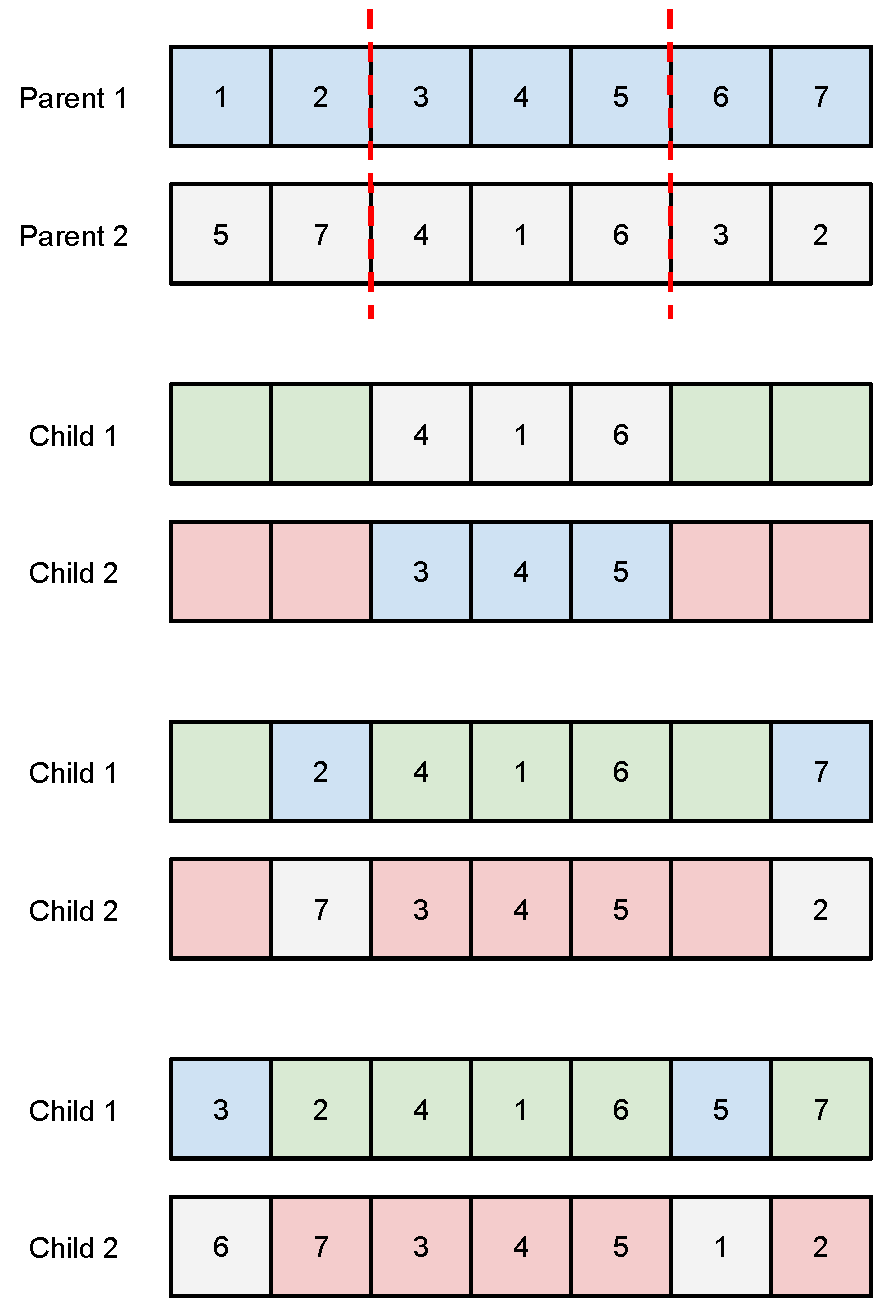
\includegraphics[width=0.7\textwidth]{Figures/recpm.pdf}
  \caption{Partially matched Crossover (recpm)}\label{fig.recpm}
\end{figure}


\paragraph{Ergebnisse}

\input{Chapters/gen/Recombination.Name}
Entscheidung: recox

